\section{Method}
\label{sec:method}

Figure~\ref{fig:architecture} summarizes \textsc{FinOPD}. The system converts raw charts into structured geometry, routes a compact alpha-factor subset, coordinates five specialist agents through shared memory, and updates itself through two complementary tracks: parametric distillation and non-parametric belief consolidation.
% 中文翻译：图 \ref{fig:architecture} 总结了 \textsc{FinOPD}。系统首先将原始图表观测转化为结构化几何表示，然后路由出紧凑的 alpha 因子子集，通过共享记忆协调五个专家智能体，最后通过双轨自进化循环更新自身：参数化在线策略蒸馏与非参数 belief 固化。

\begin{figure*}[t]
\centering
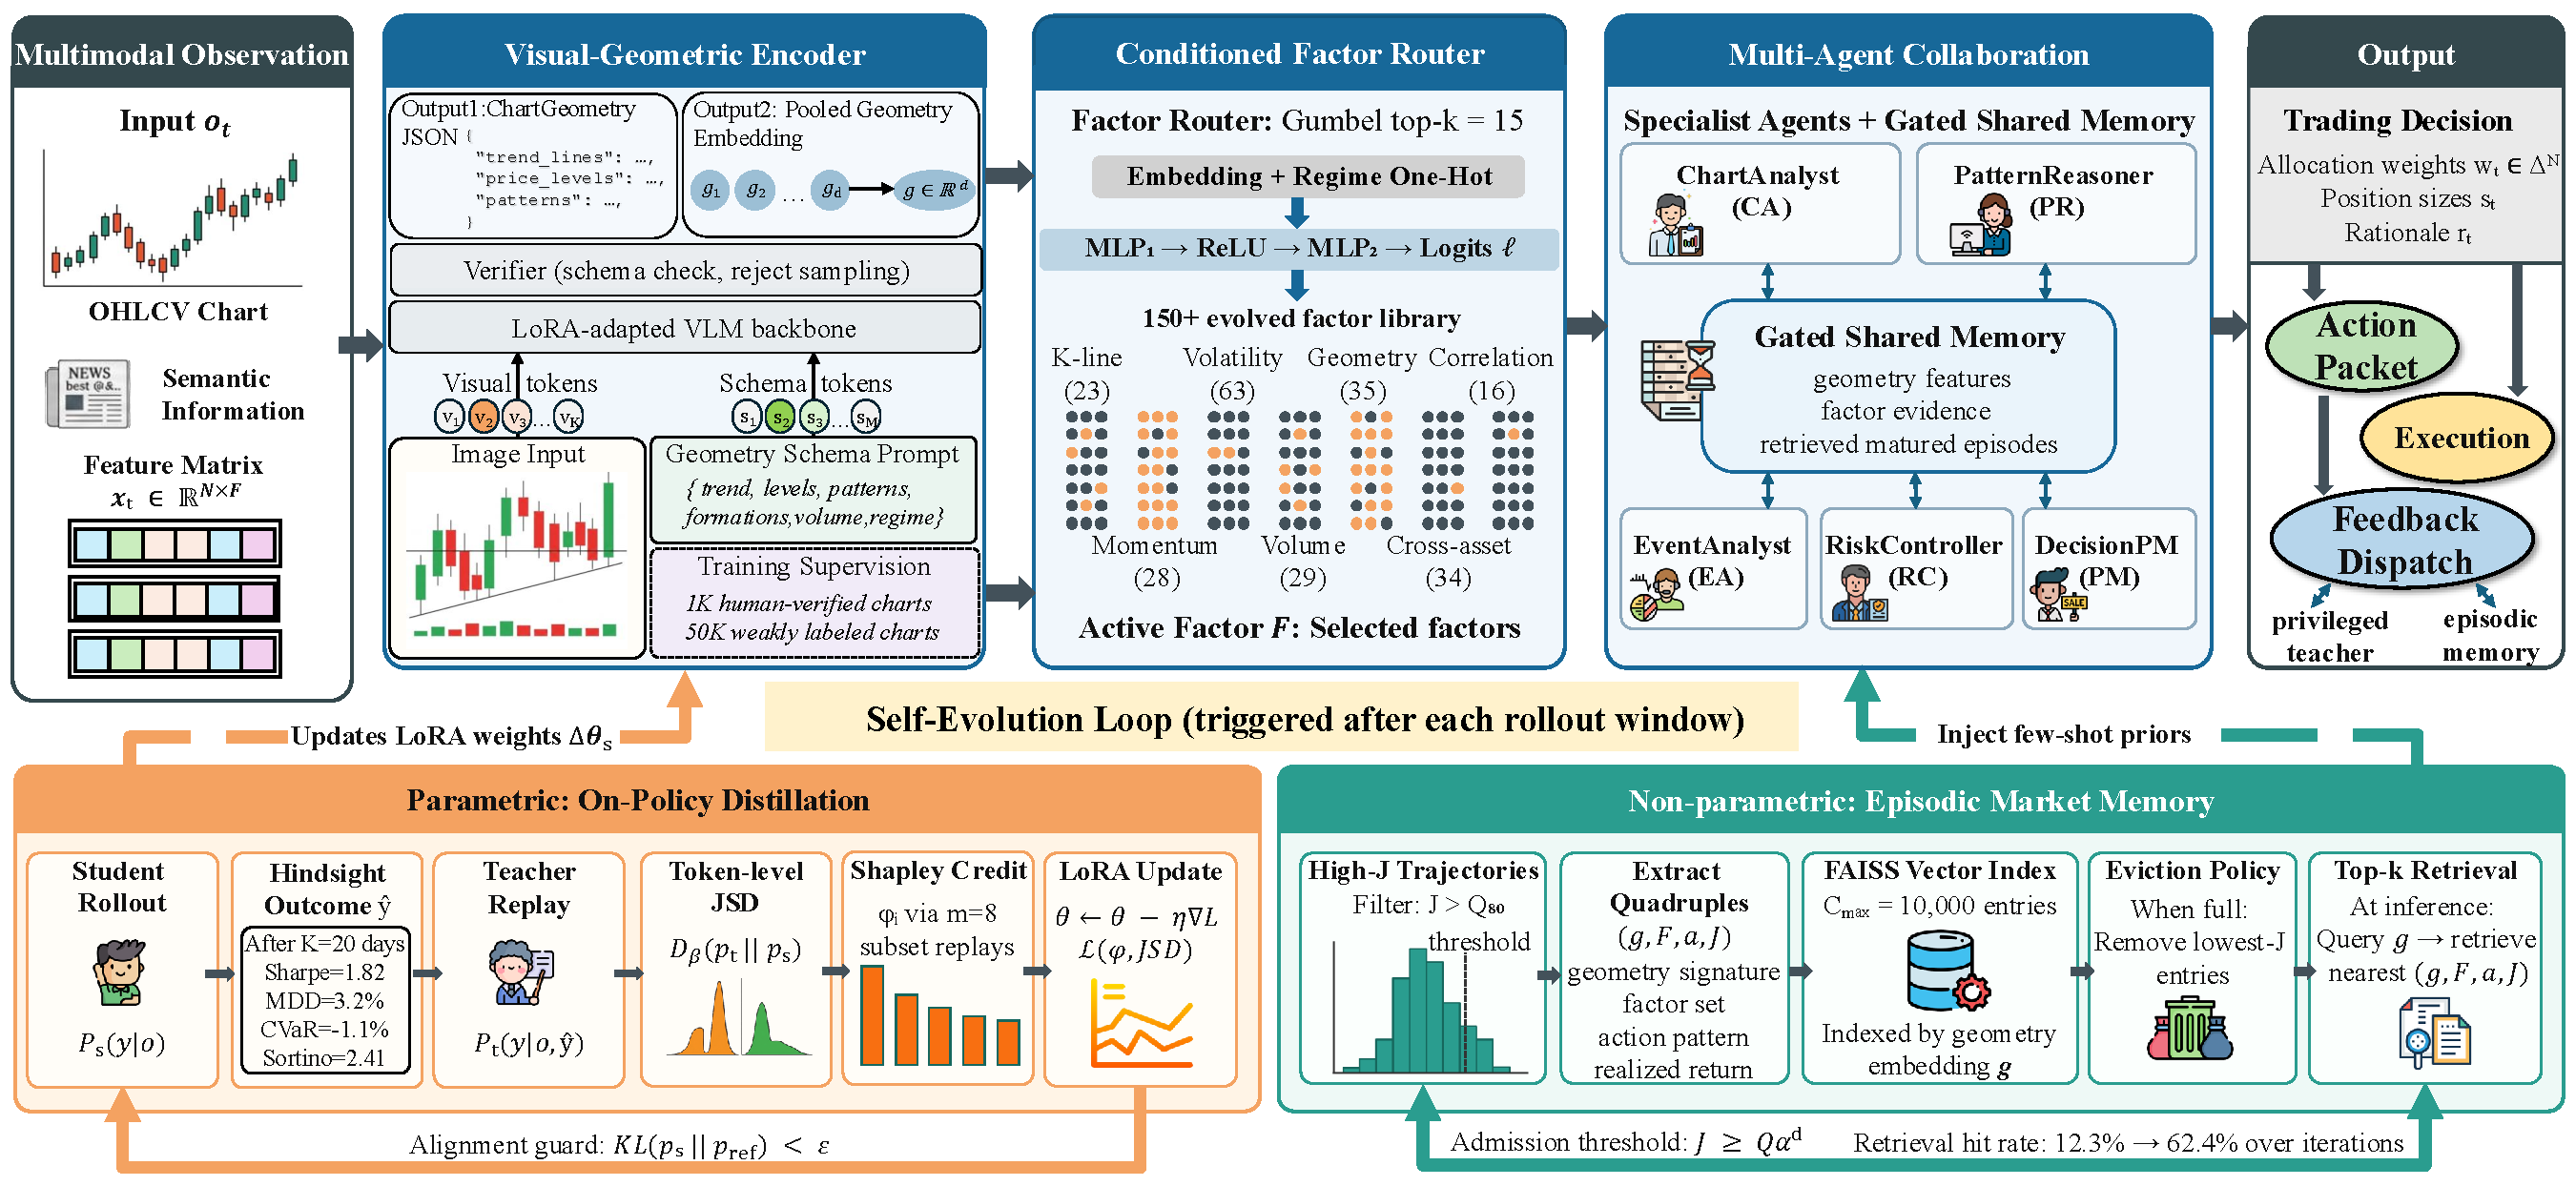
\includegraphics[width=\linewidth]{figures/FinOPD_framework.pdf}
\caption{Architecture of \textsc{FinOPD}. The Visual-Geometric Encoder extracts structured ChartGeometry from candlestick charts. The Factor Router selects factors from the candidate library via Gumbel top-$k$. Five specialist agents collaborate through gated shared memory. The dual-track self-evolution loop updates LoRA parameters via on-policy self-distillation with hindsight PnL and Shapley credit, while consolidating winning patterns into a belief store.}
% 中文翻译：\textsc{FinOPD} 架构。Visual-Geometric Encoder 从 K 线图中提取结构化 ChartGeometry；Factor Router 通过 Gumbel top-$k$ 从候选库中选择因子；五个专家智能体通过门控共享记忆协作；双轨自进化循环一方面通过带有事后 PnL 和 Shapley 信用的在线策略自蒸馏更新 LoRA 参数，另一方面把获胜模式固化到 belief store 中。
\Description{Pipeline diagram showing visual-geometric encoding, factor routing, multi-agent collaboration, and dual-track self-evolution.}
\label{fig:architecture}
\end{figure*}

\subsection{Visual-Geometric Encoder}
\label{sec:vge}

We adapt Qwen2.5-VL-7B~\cite{qwen25vl2024} with LoRA (rank 16 on the top vision layers and cross-attention modules) to output a structured \texttt{ChartGeometry} JSON. The schema contains trend lines, support--resistance levels, candlestick patterns, chart formations, volume signals, and regime state. Training uses approximately 50{,}000 US equity daily charts weakly labeled by a rule-based geometric extractor and 1{,}000 human-verified samples. A schema validator performs reject sampling and enforces structural compliance before downstream modules consume the geometry.
% 中文翻译：我们使用 LoRA（rank 16，作用于视觉顶层和交叉注意力模块）适配 Qwen2.5-VL-7B，使其输出结构化的 \texttt{ChartGeometry} JSON。该 schema 包含趋势线、支撑--阻力位、K 线形态、图表形态、成交量信号和 regime 状态。训练使用约 50,000 张由规则几何提取器弱标注的美股日线图，以及 1,000 张人工验证样本。Schema 验证器执行 reject sampling，并在下游模块消费几何信息前强制结构合规。

The encoder returns two representations. The first is an interpretable JSON object used by the agents for reasoning. The second is a pooled geometric embedding $\mathbf{g} \in \mathbb{R}^d$ from final-layer geometry tokens, used both as the conditioning signal for factor routing and as the retrieval key for the belief store.
% 中文翻译：编码器返回两种表示。第一种是可解释 JSON 对象，供智能体推理使用；第二种是来自末层几何 token 的池化几何嵌入 $\mathbf{g}\in\mathbb{R}^d$，既作为因子路由的条件信号，也作为 belief store 的检索键。

\subsection{Geometry-Conditioned Factor Router}
\label{sec:router}

The factor library $\mathcal{F}=\{f_1,\ldots,f_M\}$ contains roughly 160 candidate alpha factors, combining pre-mined LLM-evolved factors and standard technical indicators. The router maps the current geometric state to a small active subset, so the agents reason over factors that are relevant to the present market structure rather than over the entire library.
% 中文翻译：因子库 $\mathcal{F}=\{f_1,\ldots,f_M\}$ 包含约 160 个候选 alpha 因子，结合了预挖掘的 LLM 进化因子和标准技术指标。路由器将当前几何状态映射到一个小规模活跃子集，使智能体只围绕与当前市场结构相关的因子推理，而不是处理整个因子库。

Given geometry embedding $\mathbf{g}$ and regime vector $\mathbf{r}$, the router maps $[\mathbf{g};\mathbf{r}]$ to logits $\boldsymbol{\ell}\in\mathbb{R}^M$ with a two-layer MLP and applies a Gumbel-Softmax relaxation:
\begin{equation}
\label{eq:gumbel}
z_j = \frac{\exp((\ell_j + g_j) / \tau)}{\sum_{j'=1}^{M} \exp((\ell_{j'} + g_{j'}) / \tau)}, \quad g_j \sim \mathrm{Gumbel}(0, 1).
\end{equation}
The top-$k$ indices ($k{=}15$) define the active factor set $F_t\subset\mathcal{F}$. Selected factors are computed and written into the shared memory. The router is updated with a lightweight group-relative objective inside the self-evolution loop (\S\ref{sec:opsd}).
% 中文翻译：给定几何嵌入 $\mathbf{g}$ 和 regime 向量 $\mathbf{r}$，路由器用两层 MLP 计算 logits，再应用 Gumbel-Softmax 松弛。Top-$k$ 索引（$k=15$）定义活跃因子集 $F_t\subset\mathcal{F}$。被选中的因子会被计算并写入共享记忆。路由器在自进化循环内部通过轻量级 group-relative 目标更新。

\subsection{Self-Distillation with Hindsight PnL}
\label{sec:opsd}

\textsc{FinOPD} lets the same base model (Qwen3.5-9B~\cite{qwen35_2026}, LoRA rank 16) play two roles under different information conditions. The student sees only decision-time observations, while the teacher additionally sees realized risk-adjusted returns after the decision window. This differential conditioning makes hindsight PnL the privileged signal without introducing an external oracle.
% 中文翻译：\textsc{FinOPD} 让同一个基础模型在不同信息条件下扮演两个角色。学生只能看到决策时刻可得的观测，而教师额外看到决策窗口之后的已实现风险调整收益。这种差异条件化使事后 PnL 成为特权信号，而无需引入外部 oracle。

\begin{figure}[t]
\centering
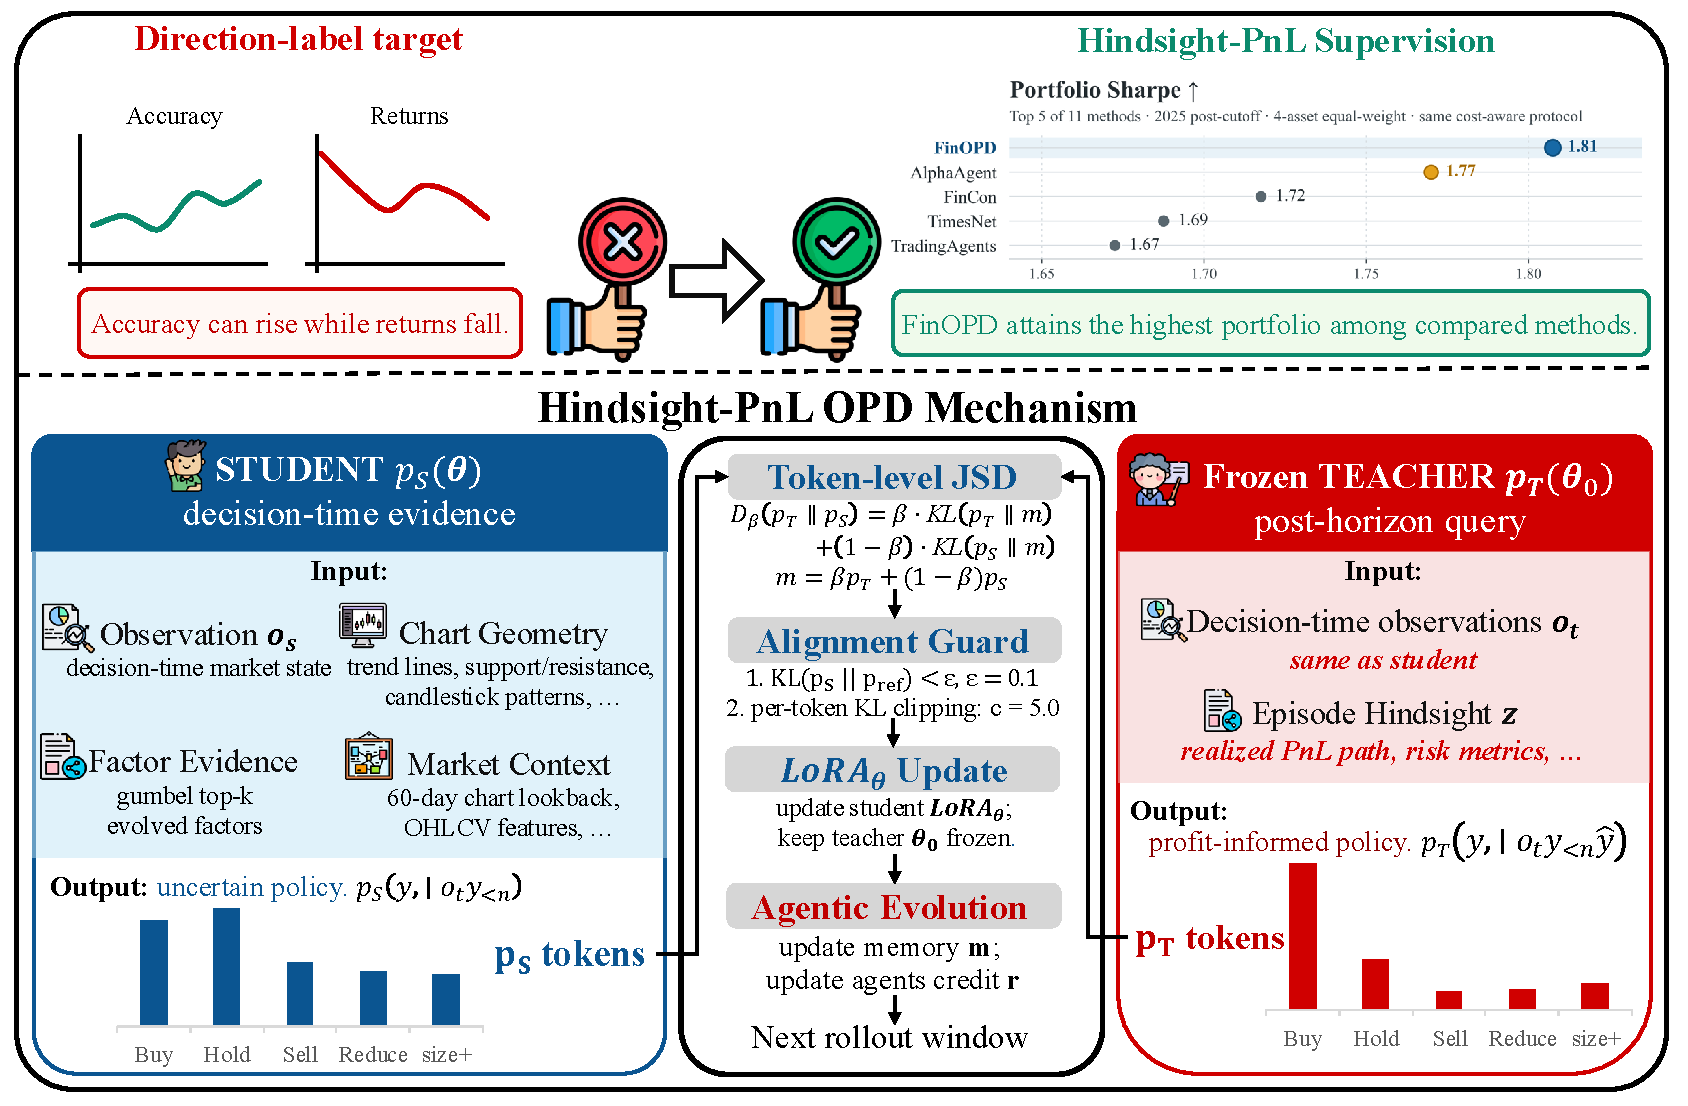
\includegraphics[width=\columnwidth]{figures/FinOPD_mechanism.pdf}
\caption{On-policy self-distillation. The same base model defines a student conditioned on $o_t$ and a frozen teacher conditioned on $o_t$ plus hindsight PnL. Token-level JSD with Shapley weighting drives parametric evolution.} %The student is the trainable policy updated by Shapley-weighted token-level JSD from decision-time evidence, while the frozen teacher sees the same evidence plus hindsight risk-adjusted PnL and serves only as the privileged distillation target.
% 中文翻译：在线策略自蒸馏。同一基础模型定义一个条件化于 $o_t$ 的学生，以及一个条件化于 $o_t$ 和事后 PnL 的冻结教师。带有 Shapley 加权的 token 级 JSD 推动参数进化。
\Description{Diagram contrasting the student conditioned on current observations with the teacher conditioned on hindsight PnL.}
\label{fig:opsd}
\end{figure}

\paragraph{Formulation.}
Let $o_t$ denote the observation at time $t$. Agent $i$ produces a sequence $y^{(i)}_t=(y^{(i)}_{t,1},\ldots,y^{(i)}_{t,L})$. Student and teacher distributions are:
\begin{align}
p_S(y^{(i)}_{t,n} \mid o_t, y^{(i)}_{t,<n}) &\quad \text{(student)}, \\
p_T(y^{(i)}_{t,n} \mid o_t, y^{(i)}_{t,<n}, \hat{y}) &\quad \text{(teacher)},
\end{align}
where $\hat{y}$ serializes realized risk statistics over the subsequent $K{=}20$ trading days, including Sharpe, MDD, CVaR, and Sortino. The teacher is frozen at the initial checkpoint, while the student LoRA parameters are updated.
% 中文翻译：设 $o_t$ 表示 $t$ 时刻的观测。智能体 $i$ 产生序列 $y^{(i)}_t$。学生分布仅条件化于 $o_t$ 和历史 token，教师分布额外条件化于 $\hat{y}$，其中 $\hat{y}$ 序列化后续 $K=20$ 个交易日的已实现风险统计，包括 Sharpe、MDD、CVaR 和 Sortino。教师冻结在初始 checkpoint，学生 LoRA 参数则被更新。

\paragraph{Training objective.}
At each token position, we minimize a generalized Jensen--Shannon divergence:
\begin{equation}
\begin{split}
D_\beta(p_T \| p_S) &= \beta\,\mathrm{KL}(p_T\|m)
 +(1{-}\beta)\,\mathrm{KL}(p_S\|m),\\
m &= \beta p_T+(1{-}\beta)p_S.
\end{split}
\end{equation}
We additionally clip per-token KL contributions,
\begin{equation}
\mathrm{KL}_{\mathrm{clip}}(n)=\sum_{v=1}^{V}
\min\left(p_T(v|n)\log\frac{p_T(v|n)}{p_S(v|n)},\;c\right),
\end{equation}
so that stylistic tokens cannot dominate the learning signal.
% 中文翻译：在每个 token 位置，我们最小化广义 Jensen--Shannon 散度，并额外裁剪逐 token KL 贡献，使风格性 token 不会主导学习信号。

\paragraph{Shapley credit assignment.}
For each high-reward trajectory, we sample $m{=}8$ random agent subsets and perform leave-subset-out replay to estimate marginal contributions $\phi_i$. The normalized Shapley values weight each agent's distillation loss, strengthening the update for agents whose outputs were more responsible for the realized outcome.
% 中文翻译：对每条高奖励轨迹，我们采样 $m=8$ 个随机智能体子集，并执行 leave-subset-out replay 来估计边际贡献 $\phi_i$。归一化 Shapley 值用于加权每个智能体的蒸馏损失，从而强化那些对已实现结果贡献更大的智能体更新。

\paragraph{Router update and alignment guard.}
Factor selection is optimized separately as a discrete action. Within a mini-batch, trajectory $j$ receives advantage $J_j-\bar{J}$, avoiding an additional critic network. To limit policy drift, we maintain $\mathrm{KL}(p_S\|p_{\mathrm{ref}})<\epsilon$ against a reference policy and refresh the training pool every four iterations with adversarial regime-shift samples, including the 2020 COVID crash and the 2022 bear market.
% 中文翻译：因子选择作为离散动作单独优化。在一个 mini-batch 内，轨迹 $j$ 的优势为 $J_j-\bar{J}$，因此不需要额外 critic 网络。为限制策略漂移，我们维持学生相对参考策略的 KL 小于 $\epsilon$，并每四轮用对抗性 regime-shift 样本刷新训练池，包括 2020 年 COVID 崩盘和 2022 年熊市。

The complete self-evolution loop is summarized in Algorithm~\ref{alg:finopd}.
% 中文翻译：完整的自进化循环见算法 \ref{alg:finopd}。

\begin{algorithm}[t]
\caption{\textsc{FinOPD} Self-Evolution (One Iteration)}
\label{alg:finopd}
\begin{algorithmic}[1]
\REQUIRE Student $p_S(\theta)$, frozen teacher $p_T(\theta_0)$, router $\pi_R$, belief store $\mathcal{B}$, window $\mathcal{W}$
\FOR{each day $t \in \mathcal{W}$}
\STATE $\mathbf{g}_t \leftarrow \mathrm{VGE}(I_t)$; retrieve priors from $\mathcal{B}$ via $\mathbf{g}_t$
\STATE $F_t \leftarrow \pi_R(\mathbf{g}_t, \mathrm{regime}_t)$ \hfill $\triangleright$ Gumbel top-$k$
\FOR{agent $i = 1 \ldots 5$}
\STATE $y^{(i)}_t \sim p_S(\cdot \mid o_t, F_t)$
\ENDFOR
\ENDFOR
\STATE $J \leftarrow \mathrm{RiskAdjPnL}(\tau)$; \ $\hat{y} \leftarrow \mathrm{serialize}(J)$
\STATE Compute $p_T(\cdot \mid o, y_{<n}, \hat{y})$ at all positions
\STATE $\{\phi_i\} \leftarrow \mathrm{ShapleyCredit}(\tau, m{=}8)$
\STATE $\mathcal{L} \leftarrow \sum_n \phi_{i(n)} \cdot D_\beta(p_T \| p_S)|_n$ with per-token KL clip
\STATE $\theta \leftarrow \theta - \eta \nabla_\theta \mathcal{L}$; \ update $\pi_R$ with group-relative advantage
\IF{$J > Q_{80}(\text{history})$}
\STATE Insert $(\mathbf{g}, F, a, J)$ into $\mathcal{B}$
\ENDIF
\IF{$\mathrm{KL}(p_S \| p_\mathrm{ref}) > \epsilon$}
\STATE Roll back $\theta$ to last safe checkpoint
\ENDIF
\RETURN Updated $\theta$, $\pi_R$, $\mathcal{B}$
\end{algorithmic}
\end{algorithm}

\subsection{Long-Term Belief Consolidation}
\label{sec:belief}

Parametric updates capture global adaptation but can dilute recurring local patterns through averaging. We therefore maintain a non-parametric belief store that preserves high-value market situations as concrete retrieval targets.
% 中文翻译：参数更新能够捕捉全局适应，但也可能通过平均稀释反复出现的局部模式。因此，我们维护一个非参数 belief store，将高价值市场情境保留为具体检索目标。

From trajectories whose $J$ exceeds the 80th percentile, we extract quadruples $(\mathbf{g},F,a,J)$: geometry signature, selected factor set, action pattern, and realized return. These entries are indexed by $\mathbf{g}$ in a FAISS vector store with capacity constraint
\begin{equation}
|\mathcal{B}| \leq C_{\max}, \quad \forall\,(\mathbf{g},F,a,J)\in\mathcal{B}:\; J \geq Q_{\alpha}(\{J_i\}_{i=1}^{|\mathcal{B}|}),
\end{equation}
where $C_{\max}=10{,}000$ and $\alpha=0.8$. When capacity is reached, the lowest-$J$ entries are evicted. At inference, the current geometry signature retrieves the top-5 nearest neighbors, and the associated $(F,a)$ pairs are injected into shared memory as few-shot priors.
% 中文翻译：对于 $J$ 超过 80 分位的轨迹，我们抽取四元组 $(\mathbf{g},F,a,J)$：几何签名、选中因子集、动作模式和已实现收益。这些条目按 $\mathbf{g}$ 索引到带容量约束的 FAISS 向量库中，其中 $C_{\max}=10,000$ 且 $\alpha=0.8$。达到容量上限时，最低 $J$ 条目会被驱逐。推理时，当前几何签名检索 top-5 近邻，相关 $(F,a)$ 对作为 few-shot 先验注入共享记忆。

The two tracks address different failure modes. The parametric track changes how the model reasons across states; the belief store recalls what worked in specific states. The ablations in \S\ref{sec:experiments} show that the full system outperforms either track alone.
% 中文翻译：两条轨道解决不同失效模式。参数轨道改变模型跨状态推理的方式；belief store 回忆特定状态下曾经有效的做法。\S\ref{sec:experiments} 中的消融显示，完整系统优于任一单独轨道。

\subsection{Regime-Adaptive Decision with Edge-Gated Abstention}
\label{sec:rasw}

The final component is motivated by a simple empirical observation: the system's edge is regime-dependent. Structured geometry and factor signals are useful when the market trends or volatility expands, but can degrade into noise in calm, directionless conditions. Trading through no-edge regimes consumes alpha through costs and slippage, so the policy must learn not only what to trade but also when not to trade.
% 中文翻译：最后一个组件来自一个简单经验观察：系统的边际优势具有 regime 依赖性。结构化几何与因子信号在市场趋势明确或波动扩大时有用，但在平静、无方向条件下可能退化为噪声。在无优势 regime 中交易会通过成本和滑点消耗 alpha，因此策略不仅要学习交易什么，还要学习什么时候不交易。

\paragraph{Regime-Adaptive Signal Weighting (RASW).}
The decision module fuses trend, factor, and mean-reversion signals through regime-conditioned weights. Let $\rho_t$ be detected from 20-day realized volatility $\sigma_t$ and 20-day trend slope $s_t$:
\begin{equation}
\label{eq:rasw}
(w_{\mathrm{trend}}, w_{\mathrm{factor}}, w_{\mathrm{mr}}) =
\begin{cases}
(0.3,\,1.0,\,0.6) & \sigma_t > \sigma_{\mathrm{hi}} \;\; \text{(volatile)} \\
(1.1,\,0.5,\,0.0) & |s_t| > s_{\mathrm{hi}} \;\; \text{(trending)} \\
(0.6,\,0.9,\,0.0) & \sigma_t < \sigma_{\mathrm{lo}} \;\; \text{(calm)} \\
(0.7,\,0.8,\,0.0) & \text{otherwise.}
\end{cases}
\end{equation}
In volatile regimes, $b_{\mathrm{mr}}=-\mathrm{clip}(4\Delta_{\mathrm{sma}},-1,1)$ fades extreme deviations from the 20-day moving average. In trending regimes, trend evidence receives the largest weight.
% 中文翻译：决策模块通过 regime 条件化权重融合趋势、因子和均值回复信号。$\rho_t$ 由 20 日已实现波动率 $\sigma_t$ 和 20 日趋势斜率 $s_t$ 检测得到。在高波动 regime 中，均值回复项 $b_{\mathrm{mr}}$ 用于衰减相对 20 日均线的极端偏离；在趋势 regime 中，趋势证据获得最大权重。

\paragraph{Edge-Gated Abstention (EGA).}
Beyond reweighting signals, \textsc{FinOPD} gates the decision to act. Let $\nu_t$ be the weighted sum of trend, factor, and mean-reversion scores. The policy opens a position only when conviction clears a regime-dependent threshold:
\begin{equation}
\label{eq:ega}
\begin{gathered}
a_t =
\begin{cases}
\textsc{Buy} & \nu_t > \theta^{+}(\rho_t), \\
\textsc{Sell} & \nu_t < \theta^{-}(\rho_t), \\
\textsc{Hold} & \text{otherwise},
\end{cases}\\
(\theta^{+},\theta^{-})=
\begin{cases}
(0.15,-0.25) & \text{edge regime}, \\
(0.60,-0.70) & \text{no-edge regime.}
\end{cases}
\end{gathered}
\end{equation}
An edge regime satisfies $\sigma_t>\sigma_{\mathrm{hi}}$ or $|s_t|>s_{\mathrm{hi}}$. In no-edge regimes, thresholds rise sharply, causing the system to abstain unless the signal is overwhelming. This discrete-action analogue of selective prediction converts weak-signal periods into zero-exposure decisions while preserving exposure in favorable regimes.
% 中文翻译：除了重新加权信号，\textsc{FinOPD} 还门控是否行动。设 $\nu_t$ 为趋势、因子和均值回复信号的加权和，策略仅在信心超过 regime 依赖阈值时开仓。Edge regime 满足 $\sigma_t>\sigma_{\mathrm{hi}}$ 或 $|s_t|>s_{\mathrm{hi}}$。在 no-edge regime 中，阈值显著提高，使系统在信号不压倒性时主动弃权。这种 selective prediction 的离散动作类比，把弱信号时期转化为零敞口决策，同时保留有利 regime 中的风险暴露。

% \section{Method}
% \label{sec:method}

% \subsection{Staged Dual-Track Self-Evolution}

% \textsc{FinOPD} treats financial self-evolution as a staged process rather than an unconstrained online rewrite. Before policy optimization, Alpha-Factor Evolution compiles a versioned symbolic tool library. During each subsequent round, the current student generates the experience on which it is updated, while matured outcomes also populate a time-safe episodic memory. Formally,
% \begin{equation}
% \label{eq:staged_evolution}
% \begin{split}
% \mathcal F^{\star}&=\mathcal E_F(\mathcal D_{\mathrm{dev}}),\\
% (\theta_{r+1},\psi_{r+1},\mathcal M_{r+1})
% &=\mathcal E_{\mathrm{OPD}}(	heta_r,\psi_r,\mathcal M_r,
% \mathcal F^{\star},\tau_r,\boldsymbol\xi_r),
% \quad \tau_r\sim d^{\pi_{\theta_r}}.
% \end{split}
% \end{equation}
% Here, $\theta_r$ and $\psi_r$ parameterize the student and factor router, respectively; $\mathcal M_r$ is Outcome-Indexed Episodic Memory; and the admitted factor library $\mathcal F^{\star}$ remains immutable throughout all OPD rounds. This yields two complementary tracks: \emph{Parametric Policy Evolution} updates how the student reasons, whereas \emph{Non-Parametric Knowledge Evolution} preserves executable factor tools and matured, state-specific episodes outside model weights.

% Figure~\ref{fig:architecture} instantiates this lifecycle. At decision time, structured chart geometry and a routed factor subset enter a five-agent chain. Gated Shared Memory exposes evidence and disagreement within that decision, and a decision manager converts the joint state into a cost-aware portfolio action. Only after the outcome horizon closes do OPD and episodic-memory admission occur.

% \begin{figure*}[t]
% \centering
% 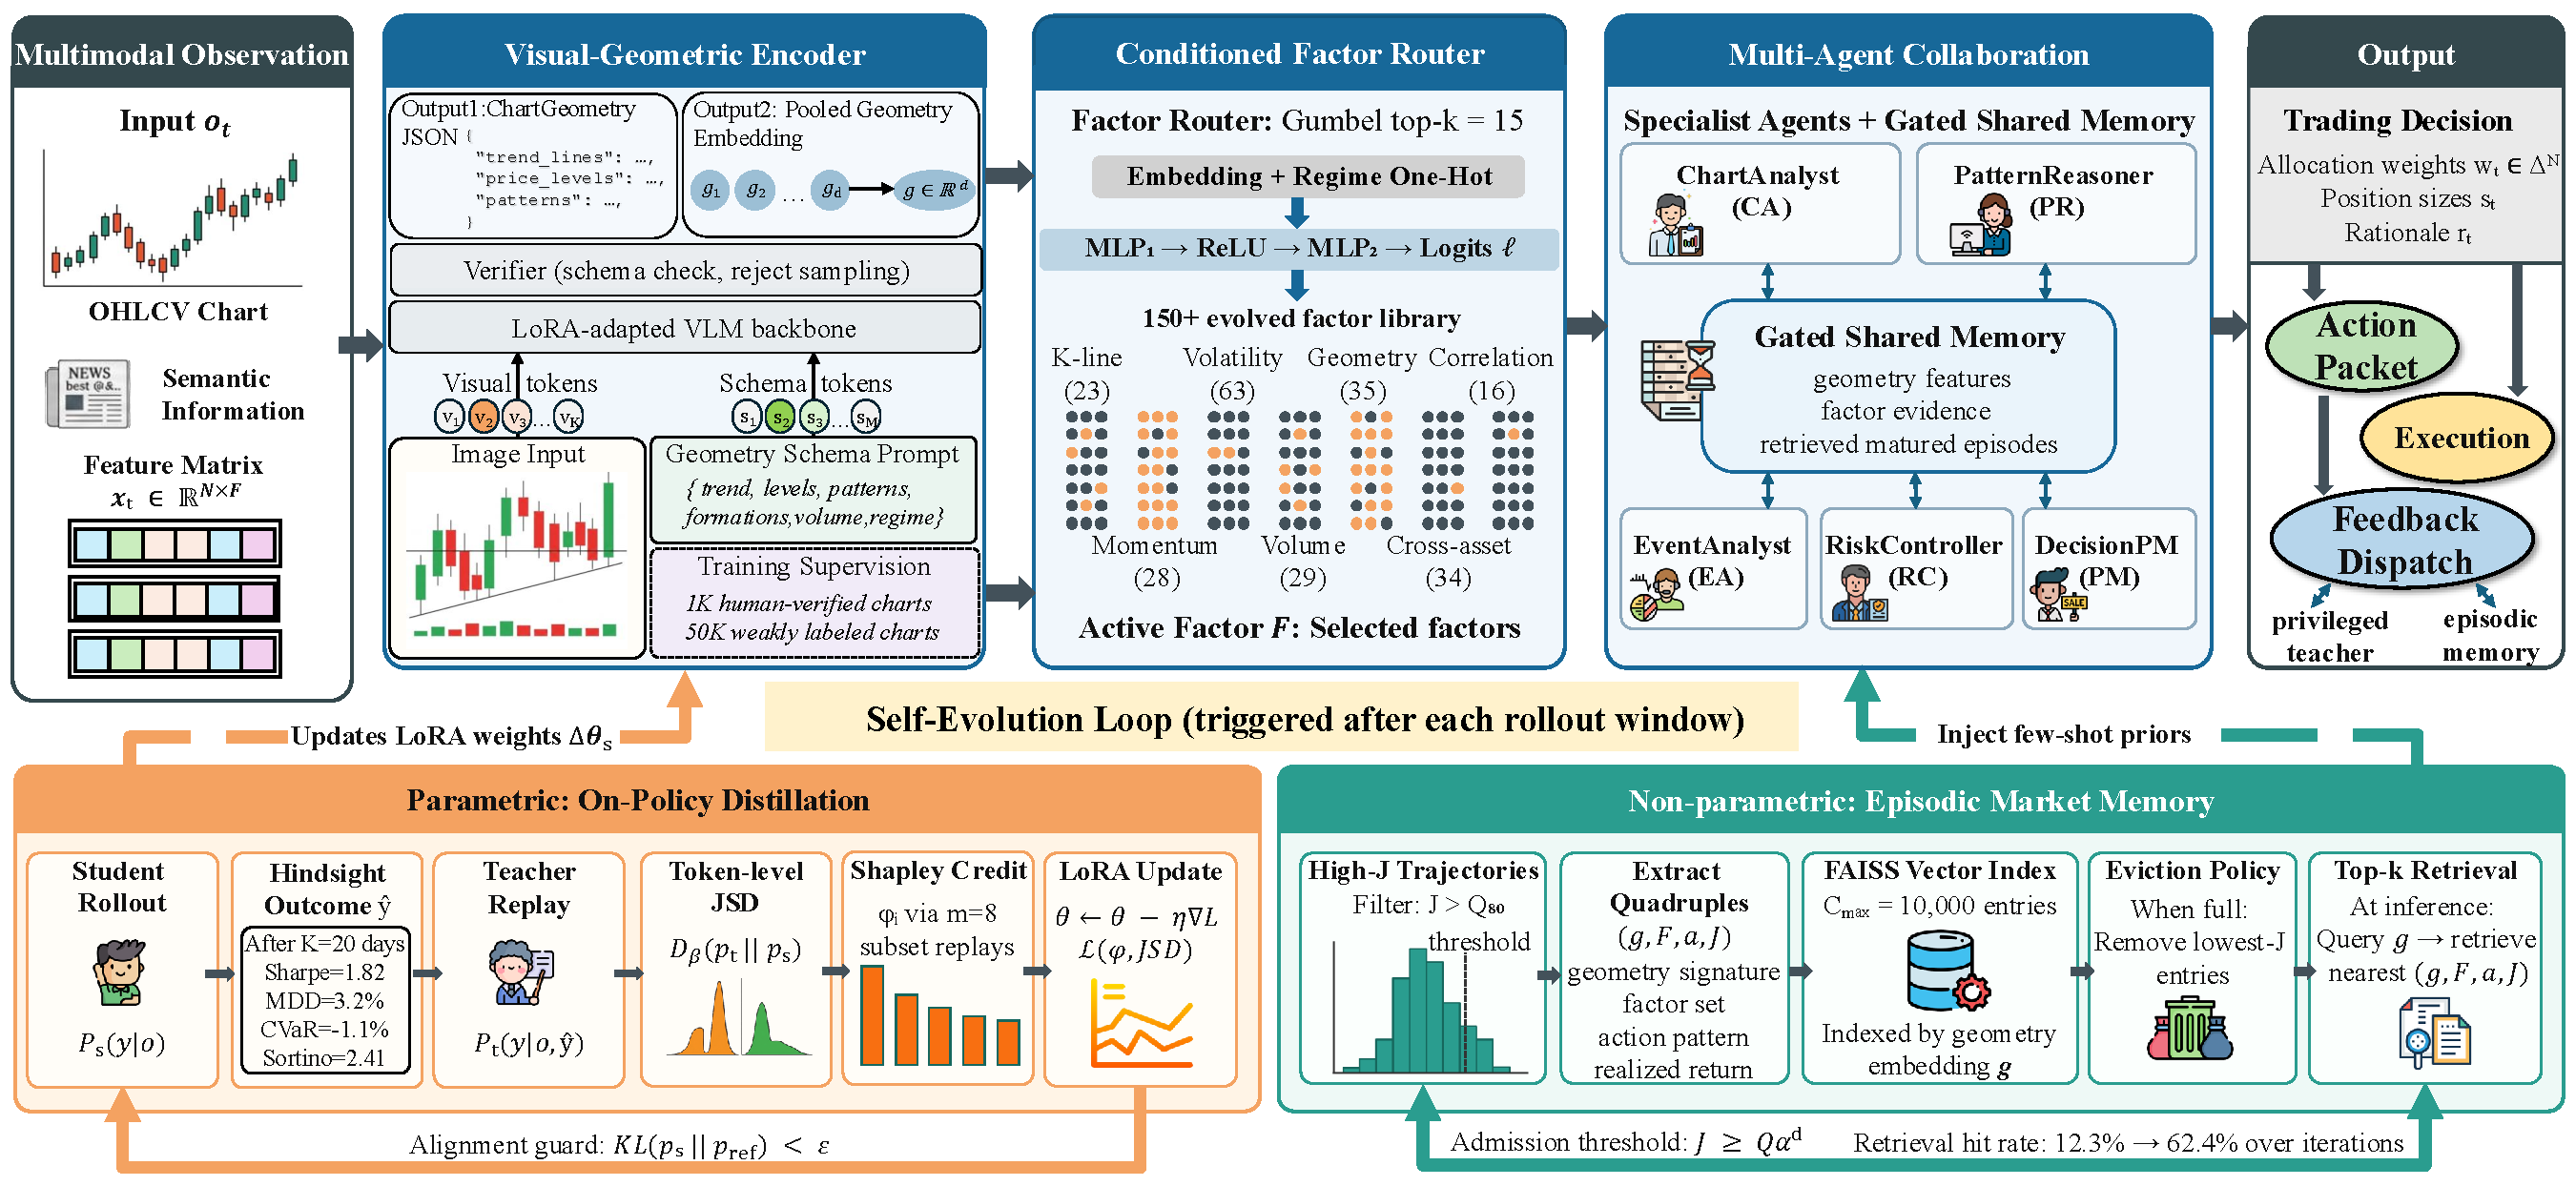
\includegraphics[width=0.99\linewidth]{figures/FinOPD_framework.pdf}
% \caption{Architecture of \textsc{FinOPD}. Alpha-Factor Evolution first constructs a fixed symbolic library. At decision time, geometry- and regime-conditioned routing supplies a compact tool subset to the five-agent decision chain. After outcomes mature, Parametric Policy Evolution updates the current student through OPD, while Non-Parametric Knowledge Evolution records time-safe outcome-indexed episodes. The factor library itself is not modified during OPD.}
% \Description{Pipeline diagram showing visual-geometric encoding, factor routing, multi-agent coordination, on-policy distillation, and non-parametric knowledge evolution.}
% \label{fig:architecture}
% \end{figure*}

% \subsection{Financial Multi-Agent Decision Backbone}

% \paragraph{Visual-geometric representation.}
% \label{sec:vge}
% The Visual-Geometric Encoder adapts Qwen2.5-VL-7B~\cite{qwen25vl2024} with rank-16 LoRA on the upper vision and cross-attention layers. It maps a point-in-time candlestick chart to a validated \texttt{ChartGeometry} object containing trend lines, support and resistance, candlestick and chart formations, volume cues, and regime descriptors. Training uses approximately 50{,}000 weakly labeled US-equity daily charts and 1{,}000 human-verified samples; malformed generations are rejected by a schema validator. The encoder returns both an auditable JSON object and a pooled geometry embedding $\mathbf g_t\in\mathbb R^d$, which conditions factor routing and episodic retrieval.

% \paragraph{Typed coordination through Gated Shared Memory.}
% The five-agent chain comprises a Chart Analyst, Pattern Reasoner, Event Analyst, Risk Controller, and Decision Manager. Their specialization is useful because their errors are asymmetric across regimes: geometric, temporal, event, and risk evidence can disagree even when each view is locally plausible. Agent $i$ therefore emits a typed message
% \begin{equation}
% \label{eq:agent_message}
% m_t^i=(e_t^i,c_t^i,a_t^i,q_t^i),
% \end{equation}
% where $e_t^i$ is supporting evidence, $c_t^i$ is confidence, $a_t^i$ is a proposed action or constraint, and $q_t^i$ records uncertainty or quality. Gated Shared Memory retains source and confidence metadata, exposes contradictions to downstream agents, and is reset for the next decision episode. Given the messages, routed factors $F_t$, retrieved episodes $E_t$, and regime $\rho_t$, the manager produces
% \begin{equation}
% \label{eq:decision_manager}
% \mathbf w_t=D_{\eta}\!\left(\{m_t^i\}_{i=1}^{A},F_t,E_t,
% \rho_t\right),
% \end{equation}
% including portfolio weights, risk constraints, and an auditable rationale. This intra-decision workspace is distinct from the cross-time memory in Section~\ref{sec:belief}.

% \subsection{Alpha-Factor Evolution and Conditional Routing}
% \label{sec:router}

% \paragraph{Pre-OPD factor evolution.}
% An LLM research process generates and mutates symbolic alpha expressions in a constrained DSL. Each candidate must parse, expose only point-in-time fields, produce finite non-constant values, and pass development-window evaluation. Candidates are ranked by cost-aware Information Ratio; invalid, duplicate, and redundant expressions are removed under a deterministic admission policy. The supplied mining stream contains 157 valid factor expressions. The resulting ordered manifest, including its required fields and content hash, defines $\mathcal F^{\star}$ and is frozen before the first OPD rollout. Thus, \emph{factor evolution} changes the library once, whereas \emph{factor routing} selects tools from that fixed library at decision time.

% \paragraph{Geometry- and regime-conditioned routing.}
% For $M=|\mathcal F^{\star}|$, let $\mathbf r_t$ embed the detected regime $\rho_t$. A two-layer router $R_{\psi}$ maps $[\mathbf g_t;\mathbf r_t]$ to logits $\boldsymbol\ell_t\in\mathbb R^M$. A Gumbel relaxation gives
% \begin{equation}
% \label{eq:gumbel}
% z_{t,j}=
% \frac{\exp((\ell_{t,j}+u_{t,j})/\tau)}
% {\sum_{j'=1}^{M}\exp((\ell_{t,j'}+u_{t,j'})/\tau)},
% \qquad u_{t,j}\sim\operatorname{Gumbel}(0,1).
% \end{equation}
% The top-$k$ entries ($k{=}15$) form $F_t\subset\mathcal F^{\star}$. Their realized values and provenance are written to Gated Shared Memory, while the manifest hash prevents index drift across rounds. The router is updated from centered trajectory utility, $U_j^H-\bar U^H$, but it never inserts, deletes, or rewrites a factor during OPD.

% \subsection{Outcome-Privileged On-Policy Distillation}
% \label{sec:opsd}

% OPD adapts the policy on the states, disagreements, and mistakes induced by its current behavior. At round $r$, $\pi_{\theta_r}$ generates $\tau_r$ using decision-time information only. After horizon $H$ closes, an estimated hindsight summary $\widehat{\mathbf h}_t^H$ is derived from the matured outcome vector $\boldsymbol\xi_t^H$. It may summarize cost-adjusted return, drawdown, CVaR, and turnover, but contains no raw future price path, OHLCV array, or future chart. A separate frozen teacher checkpoint $q_{\phi}$ receives this summary; the deployable student never does:
% \begin{align}
% \pi_{\theta}^{i,n}&=\pi_{\theta}
% (y_{t,n}^i\mid h_t^i,y_{t,<n}^i),
% \nonumber\\
% q_{\phi}^{i,n}&=q_{\phi}
% (y_{t,n}^i\mid h_t^i,y_{t,<n}^i,
% \widehat{\mathbf h}_t^H).
% \label{eq:teacher_student}
% \end{align}
% Both use the Qwen3.5-9B backbone with rank-16 LoRA~\cite{qwen35_2026}; the teacher is frozen and logically distinct from the round-start reference policy.

% \begin{figure}[t]
% \centering
% 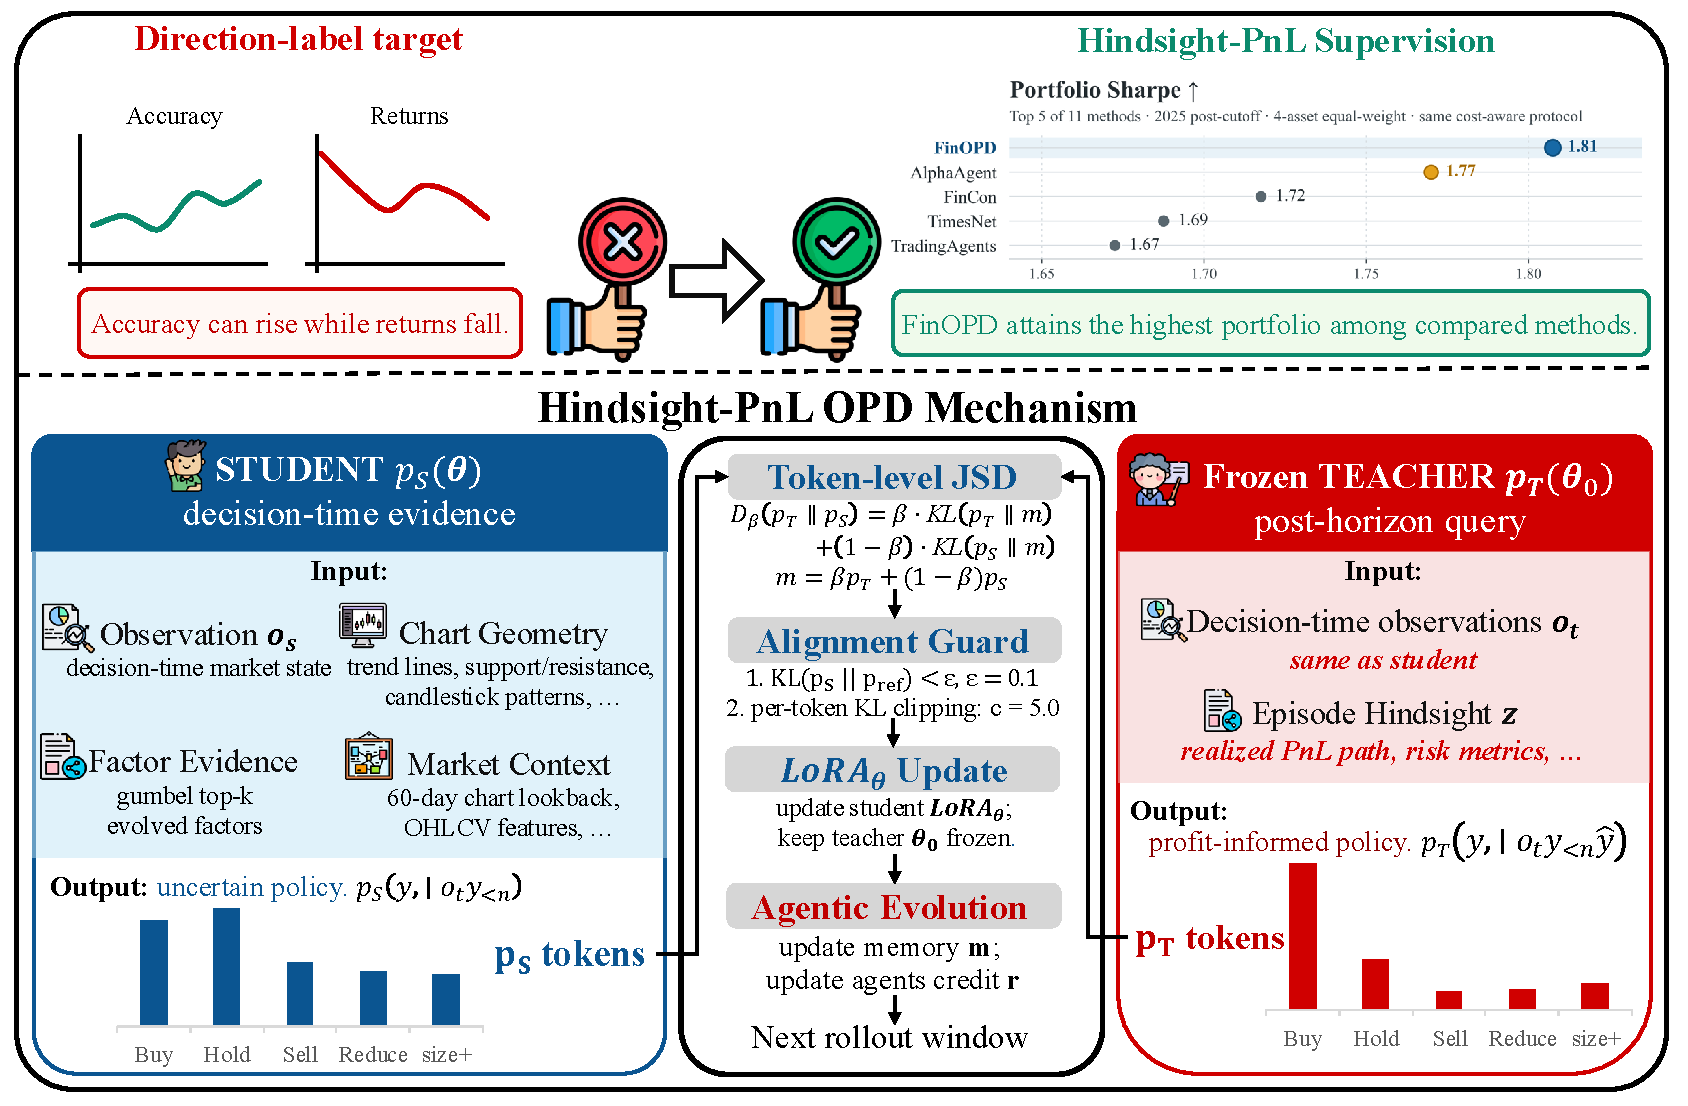
\includegraphics[width=\columnwidth]{figures/FinOPD_mechanism.pdf}
% \caption{Outcome-privileged OPD. Current-student trajectories use decision-time evidence; after outcomes mature, a separate frozen teacher additionally sees estimated hindsight. Agent-weighted token JSD and clipped teacher--student token KL drive the update, while a frozen round-start reference guards policy drift.}
% \Description{Diagram contrasting a deployable student conditioned only on current observations with a frozen teacher conditioned additionally on a derived hindsight summary.}
% \label{fig:opsd}
% \end{figure}

% \paragraph{Token-level objective and two stabilization scales.}
% For token $n$ of agent $i$, let
% \begin{align}
% \bar p_{t,i,n}
% &=\beta q_{\phi}^{i,n}+(1-\beta)\pi_{\theta}^{i,n},
% \nonumber\\
% d^{\mathrm{JS}}_{t,i,n}
% &=\beta\,D_{\mathrm{KL}}(q_{\phi}^{i,n}\|\bar p_{t,i,n})
%  +(1-\beta)D_{\mathrm{KL}}(\pi_{\theta}^{i,n}\|\bar p_{t,i,n}),
% \nonumber\\
% \widetilde k_{t,i,n}
% &=\min\!\left\{
% D_{\mathrm{KL}}(q_{\phi}^{i,n}\|\pi_{\theta}^{i,n}),c
% \right\},\qquad c=5.0.
% \label{eq:opd_token}
% \end{align}
% Crucially, the full vocabulary KL is computed for a response token before the resulting scalar is clipped; clipping signed vocabulary summands would no longer be a KL divergence. With assistant-token mask $\mu_{t,i,n}$, a non-negative utility gate $g(U_t^H)$, and normalized agent credit $\omega_{t,i}$, the OPD objective is
% \begin{equation}
% \label{eq:opd_loss}
% \mathcal L_{\mathrm{OPD}}(\theta)=
% \mathbb E_{\tau_r}\!\left[
% \sum_{t,i,n}g(U_t^H)\omega_{t,i}\mu_{t,i,n}
% \left(d^{\mathrm{JS}}_{t,i,n}
% +\lambda_{\mathrm{tok}}\widetilde k_{t,i,n}\right)
% \right].
% \end{equation}
% Here, $\lambda_{\mathrm{tok}}\geq0$ fixes the weight of the clipped token-KL term across rounds.
% This cap controls an extreme teacher--student mismatch at one response token. A separate constraint controls accumulated policy drift. Freezing $\pi_{\theta_r}$ at the beginning of round $r$, we measure
% \begin{equation}
% \label{eq:reference_kl}
% \mathcal K_{\mathrm{ref}}(\theta;\theta_r)=
% \frac{\mathbb E\!\left[
% \sum_{t,i,n}\mu_{t,i,n}
% D_{\mathrm{KL}}(\pi_{\theta}^{i,n}\|\pi_{\theta_r}^{i,n})
% \right]}{\mathbb E[\sum_{t,i,n}\mu_{t,i,n}]}
% \leq\epsilon,\qquad \epsilon=0.1.
% \end{equation}
% An optimizer step that exceeds the measured budget is skipped or rolled back. The teacher $q_{\phi}$ supplies the privileged target; $\pi_{\theta_r}$ supplies the deployment anchor. Conflating these two policies would defeat the purpose of the guard.

% \paragraph{Agent-credit weighting.}
% A trajectory-level outcome must be assigned to several interacting messages. We expose a generic credit interface through $\omega_{t,i}$ and use approximate Shapley subset replay as its current estimator. For a coalition $S$ of agents,
% \begin{align}
% \label{eq:agent_credit}
% v_t(S)
% &=U_t^H\!\left(D_{\eta}(\{m_t^j:j\in S\})\right),
% \nonumber\\
% \widehat\phi_{t,i}
% &=\frac{1}{B}\sum_{b=1}^{B}
% \left[v_t(S_b\cup\{i\})-v_t(S_b)\right],
% \end{align}
% with $B{=}8$ sampled subsets. A positive normalized transform of $\widehat\phi_{t,i}$ yields $\omega_{t,i}$. Credit therefore modulates the OPD signal without becoming a separate optimization target or requiring the credit estimator itself to be a headline contribution.

% \subsection{Outcome-Indexed Episodic Memory}
% \label{sec:belief}

% Parametric updates capture reusable behavior but can average away rare, high-value market situations. We preserve such situations as finalized episodes
% \begin{equation}
% \label{eq:episode_schema}
% e_j=(\mathbf g_j,\rho_j,F_j,\{m_j^i\},\mathbf w_j,
% \boldsymbol\xi_j^H,t_j^{\mathrm{dec}},t_j^{\mathrm{end}},
% t_j^{\mathrm{avail}}).
% \end{equation}
% An episode can be admitted only after its horizon closes,
% $t_j^{\mathrm{avail}}\geq t_j^{\mathrm{end}}>t_j^{\mathrm{dec}}$, and when its utility exceeds the historical 80th percentile. Novelty filtering removes near-duplicates; a capacity of $C_{\max}=10{,}000$ evicts the lowest-utility stale entries.

% At query time $t$, entries with $t_j^{\mathrm{avail}}>t$ are removed \emph{before} nearest-neighbor ranking. Eligible episodes are then scored by
% \begin{equation}
% \label{eq:memory_score}
% s(e_j\mid t)=
% \alpha_s\operatorname{sim}(\mathbf g_t,\mathbf g_j)
% +\alpha_r\mathbf 1[\rho_t=\rho_j]
% +\alpha_u\widetilde U_j
% +\alpha_d\operatorname{decay}(t-t_j^{\mathrm{avail}}).
% \end{equation}
% The non-negative $\alpha$ coefficients weight geometry, regime match, normalized historical utility $\widetilde U_j$, and recency.
% The top five episodes are retrieved with a FAISS index~\cite{johnson2019billion} and injected as attributed priors, not as labels. The timestamp filter prevents a backtest query from retrieving an outcome that was not yet knowable.

% \subsection{Regime-Aware Selective Execution}
% \label{sec:rasw}

% The decision layer asks when the combined evidence is tradable. Regime-Adaptive Signal Weighting (RASW) maps the messages, routed factors, and retrieved priors to a conviction score $\nu_t$ using regime-conditioned weights. Edge-Gated Abstention (EGA) then executes only when conviction clears an asymmetric regime threshold:
% \begin{equation}
% \label{eq:selective_execution}
% a_t=
% \begin{cases}
% \textsc{Buy}, & \nu_t>\kappa^+(\rho_t),\\
% \textsc{Sell}, & \nu_t<\kappa^-(\rho_t),\\
% \textsc{Hold}, & \text{otherwise}.
% \end{cases}
% \end{equation}
% The reported configuration uses $(\kappa^+,\kappa^-)=(0.15,-0.25)$ in an edge regime and $(0.60,-0.70)$ otherwise. Position sizing additionally enforces the Risk Controller's veto, transaction costs, a volatility-conditioned holding horizon, and trend-break exits. We use \emph{Regime-Aware Selective Execution} as the umbrella mechanism; RASW and EGA are local components rather than independent contribution claims.

% Algorithm~\ref{alg:finopd} summarizes the complete chronology and, in particular, makes the information boundary explicit.

% \begin{algorithm}[t]
% \caption{\textsc{FinOPD}: One Self-Evolution Round}
% \label{alg:finopd}
% \small
% \begin{algorithmic}[1]
% \REQUIRE Student $\pi_{\theta_r}$, teacher $q_{\phi}$, router $R_{\psi_r}$, frozen $\mathcal F^\star$, memory $\mathcal M_r$, horizon $H$
% \STATE Freeze reference $\pi_{\theta_r}^{\mathrm{ref}}\leftarrow\pi_{\theta_r}$
% \FOR{decision time $t$ in round $r$}
% \STATE Encode $\mathbf g_t$; retrieve eligible $E_t\leftarrow\mathcal M_r(t,\mathbf g_t,\rho_t)$
% \STATE Route $F_t\leftarrow R_{\psi_r}(\mathbf g_t,\rho_t;\mathcal F^\star)$
% \STATE Reset shared memory; collect $\{m_t^i\}$ from $\pi_{\theta_r}$
% \STATE Execute $\mathbf w_t\leftarrow D_\eta(\{m_t^i\},F_t,E_t,\rho_t)$
% \STATE Record policy, round, factor-manifest, and decision timestamps
% \ENDFOR
% \STATE Wait until $H$ closes; attach $\boldsymbol\xi_t^H$ and derive $\widehat{\mathbf h}_t^H$
% \STATE Evaluate frozen teacher and reference; estimate $\{\omega_{t,i}\}$
% \STATE Propose $(\theta',\psi')$ from Eq.~\eqref{eq:opd_loss} and centered utility
% \IF{$\mathcal K_{\mathrm{ref}}(\theta';\theta_r)\leq\epsilon$}
% \STATE Accept $\theta_{r+1}\leftarrow\theta'$ and $\psi_{r+1}\leftarrow\psi'$
% \ELSE
% \STATE Keep last safe student and router
% \ENDIF
% \STATE Admit mature, high-utility, non-duplicate episodes into $\mathcal M_{r+1}$
% \RETURN $\theta_{r+1},\psi_{r+1},\mathcal M_{r+1}$; keep $\mathcal F^\star$ fixed
% \end{algorithmic}
% \end{algorithm}
